%\chapter*{Copyright}

%This document is licensed under the Creative Commons Attribution-No Derivative Works 3.0 License. 
%To view a copy of this license, visit
%\begin{center}
%\url{http://creativecommons.org/licenses/by-nd/3.0/}.
%\end{center}

\chapter{Introduction}

ElmerGUI is a graphical user interface for the Elmer software suite
\cite{ElmerHome}. The program is capable of importing finite element mesh files in
various formats, generating finite element partitioning for various geometry
input files, setting up PDE-systems to solve, and exporting model data and results
for ElmerSolver.

ElmerGUI can also automatically call Paraview. Previously also ElmerPost and internal
VTK based postprocessors were once supported but these are gradually becoming obsolete.
%and ElmerPost to visualize. ElmerGUI has also an internal postprocessor,
%which can be used as an alternative to ElmerPost, to draw color surfaces, contours, 
%vector fields, and visualize time dependent data.

\begin{figure}[htb]
\begin{center}
 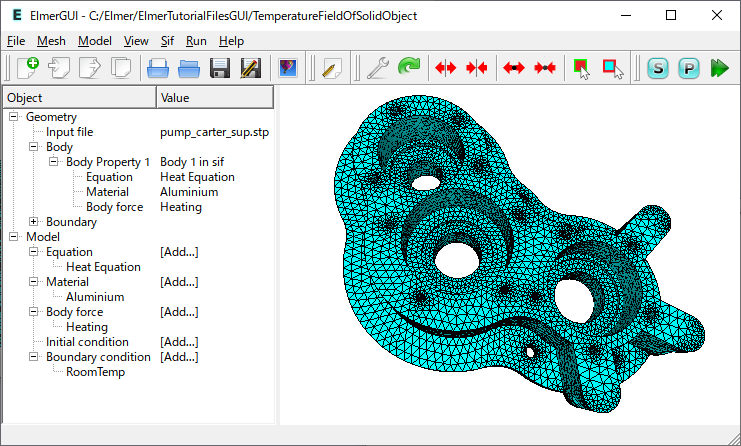
\includegraphics[scale=0.6]{images/elmergui.png}
\caption{Main window of ElmerGUI.}
\end{center}
\end{figure}

The menus of ElmerGUI are programmable and it should be relatively easy to strip and customize the interface
for proprietary applications. An example of customizing the menus is provided in appendix A.

ElmerGUI is also the interface to the parallel solver,  {\tt ElmerSolver\_mpi}.
The GUI hides from the user many operations that are normally performed from command line with
various external tools related to domain decomposition, launching the parallel processes.
This makes it possible to use ElmerSolver with multi-core processors, even on interactive
desktop environments.

ElmerGUI relies on the Qt cross platform framework of Qt Company\cite{QtHome}, and it uses the Qwt
library by Josef Wilgen and Uwe Rathman\cite{QwtHome} to plot scientific data.
%ElmerGUI relies on the Qt4 cross platform framework of QtSoftware \cite{QtHome}, and it uses the Qwt5
%library by Josef Wilgen and Uwe Rathman\cite{QwtHome} to plot scientific data.
\begin{comment}
The internal postprocessor
of ElmerGUI is based on the Visualization Toolkit (VTK) of Ken Martin, Will Schroeder, and Bill Lorensen
\cite{VTKHome}.
\end{comment}
The CAD import features are implemented by the OCE library from Open CASCADE Community Edition developers\cite{OCCHome} 
and Netgen\cite{NetgenHome} as finite element mesh generators.

%The CAD import features are implemented by the OpenCASCADE (OCC) library from
%OpenCASCADE S.A.S. \cite{OCCHome}. The program is also capable of using Tetgen \cite{TetgenHome}
%and Netgen \cite{NetgenHome} as finite element mesh generators.
\chapter{Installation from source}

The source code of ElmerGUI is available from the Git repository hosted at GitHub. The GPL
licensed source code may be downloaded by executing the command 
\begin{verbatim}
  git clone git://www.github.com/ElmerCSC/elmerfem
\end{verbatim}
or
\begin{verbatim}
  git clone https://www.github.com/ElmerCSC/elmerfem
\end{verbatim}
\noindent This will retrieve the current development version of the whole Elmer-suite.

\section{Linux}

Before starting to compile, please make sure that you have the development package of Qt
installed on your system (i.e., libraries, headers, and program development tools). Qt version 4.3
or newer is recommended. You may also wish to install Qwt 6,
VTK version 8.2,
and OCE 0.18, for additional functionality. 

CMake can be used to generate the makefiles for compilation. The compilation of ElmerGUI is activated 
in the first place by setting the corresponding CMake variable as {\tt -DWITH\_ELMERGUI:BOOL=TRUE}. 
Other logical variables that affect the compilation of the program and that can similarly be set 
%from the command line 
with {\tt -D} are {\tt WITH\_QWT}, {\tt WITH\_VTK},
{\tt WITH\_OCC}, {\tt WITH\_PYTHONQT},
{\tt WITH\_MATC} and {\tt WITH\_PARAVIEW}. {\tt WITH\_QT5} is also required when compiling with Qt5 instead of Qt4.

%The program compiled and installed by executing the following sequence of commands in a terminal window:
%\begin{verbatim}
%$ cd elmerfem/trunk/ElmerGUI
%$ qmake
%$ make
%$ make install
%\end{verbatim}
%The default installation directory defined in the project file {\tt ElmerGUI.pri} is {\tt /usr/local/bin}.

%It is possible that the project definition file ``ElmerGUI.pri'' needs to be edited and modified, depending
%on how and where the external libraries have been installed. The lines that need attention can be found from
%the beginning of the file.

Once the build process has finished, it suffices to set up the environment variable {\tt ELMERGUI\_HOME}
and add it to {\tt PATH}:
\begin{verbatim}
$ export ELMERGUI_HOME=/usr/local/bin
$ export PATH=$PATH:$ELMERGUI_HOME
\end{verbatim}
The program is launched by the command
\begin{verbatim}
$ ElmerGUI
\end{verbatim}

%Later, it is possible to update ElmerGUI by the following commands within the build directory:
%\begin{verbatim}
%$ svn update
%$ make
%$ make install
%\end{verbatim}

% =======================================================================
% CMake era: Windows compilation instructions need (?) revision.
% They are now (Oct, 2015) commented out until someone revises the text. 
% =======================================================================


%\section{Windows}

%On 32-bit Windows systems, it is possible to use precompiled binary packages, which are distributed
%through the file release system of SourceForge.NET \cite{ElmerfemHome}. The binary packages may depend
%on external components, which must be installed prior to downloading Elmer. The list of possible
%dependencies can be found from the ``Release notes'' of the package.

%It is also possible to compile ElmerGUI from source. This can be done either by
%Visual Studio 2008 C++ Express Edition \cite{VCEE2008Home} (or any other MS
%compiler that provides at least the same functionality), or by using the GNU
%Compiler Collection provided by the MinGW project \cite{MinGWHome}.

%The compilation instructions for MinGW are more or less the same as for Linux.
%The only exception is that then OCC should probably be excluded from compilation. 

%The advantage of using MinGW is that it is then possible to use Qt's precompiled
%binary packages \cite{QtHome}, which otherwise have to be built from source. MinGW
%might also be the natural choice for users that prefer Unix-like operating environments.

%The easiest way to compile ElmerGUI with VC++ is to invoke ``Visual Studio 2008 Command Prompt''
%and execute the following sequence commands within ElmerGUI's source directory:
%\begin{verbatim}
%> qmake
%> nmake
%> nmake install
%\end{verbatim}

%Again, it is necessary to verify that the search paths to all external components have been
%correctly defined in ``ElmerGUI.pri''. The build process is performed in release mode, producing
%the executable ``Application/release/ElmerGUI.exe''.

%The final task is to introduce the environment variable {\tt ELMERGUI\_HOME} with
%value {\tt c:/Elmer5.4/bin} and add it to the binary search path (right-click My Computer
%$\rightarrow$ Properties $\rightarrow$ Advanced $\rightarrow$ Environment variables)

\chapter{Input files}

\section{Geometry input files and mesh generation}

ElmerGUI is capable of importing finite element mesh files and generating two or three
dimensional finite element partitioning for bounded domains with piecewise linear
boundaries. It is possible to use one of the following mesh generators:
\begin{itemize}
 \item ElmerGrid (built-in)
 \item Tetgen (optional)
 \item Netgen (built-in)
\end{itemize}
The default import filter and mesh generator is ElmerGrid. Tetgen is an optional
module, which may or may not be available depending on the installation (installation and
compilation instructions can be found from Elmer's source tree in {\tt trunk/misc})

An import filter or a mesh generator is selected automatically by ElmerGUI when a geometry
input file is opened:

\menu{File}{Open...}

The selection is based on the input file suffix according to Table \ref{table:inputfiles}. If two or more
generators are capable of handing the same format, then the user defined ``preferred
generator'' will be used. The preferred generator is defined in

\menu{Mesh}{Configure...}

Once the input file has been opened, it is possible to modify the mesh parameters
and remesh the geometry for better accuracy or computational efficiency. The mesh parameters
can be found from $Mesh \rightarrow Configure...$. The control string for Tetgen
has been discussed and explained in detail in Tetgen's user guide \cite{TetgenHome}.

\begin{table}
	\caption{Input files and capabilities of the mesh generators.}
	\label{table:inputfiles}
	\begin{center}
		\begin{tabular}{|c|c|c|c|}
		\hline
		 Suffix & ElmerGrid & Tetgen & Netgen \\
		\hline 
		.FDNEUT & yes & no & no \\
		.grd  & yes & no & no \\
		.msh & yes & no & no \\
		.mphtxt & yes & no & no \\
		.off & no & yes & no \\
		.ply & no & yes & no \\
		.poly & no & yes & no \\
		.smesh & no & yes & no \\
		.stl  & no & yes & yes \\
		.unv & no & yes & no \\
		.in2d & no & no & yes \\
		\hline
		\end{tabular}
	\end{center}
\end{table}

The mesh generator is reactivated from the Mesh menu by choosing

\menu{Mesh}{Remesh}
\noindent In case of problems, the meshing thread may be terminated by executing 
\menu{Mesh}{Terminate meshing}

\section{Elmer mesh files}

An Elmer mesh consists of the following four text files (detailed description of the file
format can be found from Appendix B):

\begin{footnotesize}
\begin{verbatim}
mesh.header 
mesh.nodes 
mesh.elements 
mesh.boundary 
\end{verbatim}
\end{footnotesize}

Elmer mesh files may be loaded and/or saved by opening the mesh directory from the File menu:
\menu{File}{Load mesh...}
\noindent and/or
\menu{File}{Save as...}

\section{Project files}

An ElmerGUI project consists of a project directory containing Elmer mesh files and an xml-formatted 
document {\tt egproject.xml} describing the current state and settings. These files will be generated or updated when you save your project by choosing

\menu{File}{Save project}

This will save your project to the project directory you already specified. (If no project directory is specified yet, a window will appear to specify the project directory.) If you want to save your project in different directory, you can do that by choosing

\menu{File}{Save project as...}

\noindent Projects you already saved may be loaded by choosing

\menu{File}{Load project...}

\noindent or you can simply select one from

\menu{File}{Recent projects}
\vspace{3mm}
\noindent {\bf Note}: Current version of ElmerGUI has a menu to start a new project \menu{File}{New project...}
 \noindent and by clicking the menu, a window will appear to specify project directory for the new project. You can also specify Elmer mesh directory or geometry input file you want to load for the project. Extra equation definition files can be also specified in the same window. This menu is just for convenience and previous style of workflow (i.e. open geometry input file, set conditions, then save project) still works.

\vspace{3mm}
The contents of a typical project directory are the following:

\begin{footnotesize}
	\begin{verbatim}
	case.sif 
	egproject.xml
	ELMERSOLVER_STARTINFO 
	mesh.boundary 
	mesh.elements 
	mesh.header 
	mesh.nodes
	\end{verbatim}
\end{footnotesize}

\chapter{Model definitions}

\section{Setup menu}

The general setup menu can be found from
\menu{Model}{Setup...}
\noindent This menu defines the basic variables for the ``Header'', ``Simulation'',
and ``Constants'' blocks for a solver input file. The contents of these blocks have
been discussed in detail in the SolverManual of Elmer \cite{ElmerHome}.

\begin{figure}[htb]
\begin{center}
 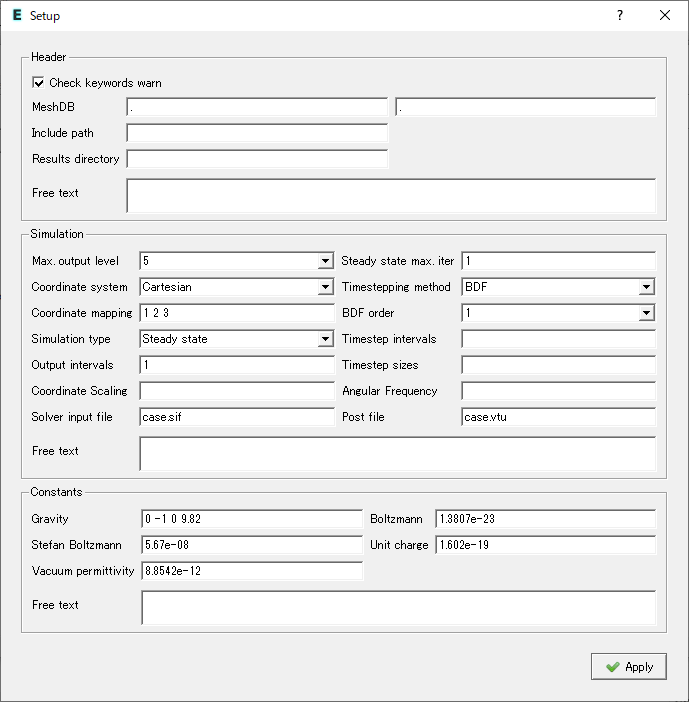
\includegraphics[scale=0.5]{images/setupmenu.png}
\caption{Setup Window.}
\end{center}
\end{figure}

\section{Equation menu}

The first ``dynamical menu'' constructed from the ElmerGUI definition files (see Appendix A) is
\menu{Model}{Equation}
\noindent This menu defines the PDE-system to be solved as well as the numerical
methods and parameters used in the solution. It will be used to generate the ``Solver''
blocks in a solver input file.

A PDE-system (a.k.a ``Equation'') is defined in a Equation Window which shows up by choosing
\dynmenu{Model}{Equation}{Add...}

\noindent or clicking [Add...] label next to ``Equation'' item in Object Browser as shown in Figure \ref{fig:equation}.

\begin{figure}[htb]
\begin{center}
 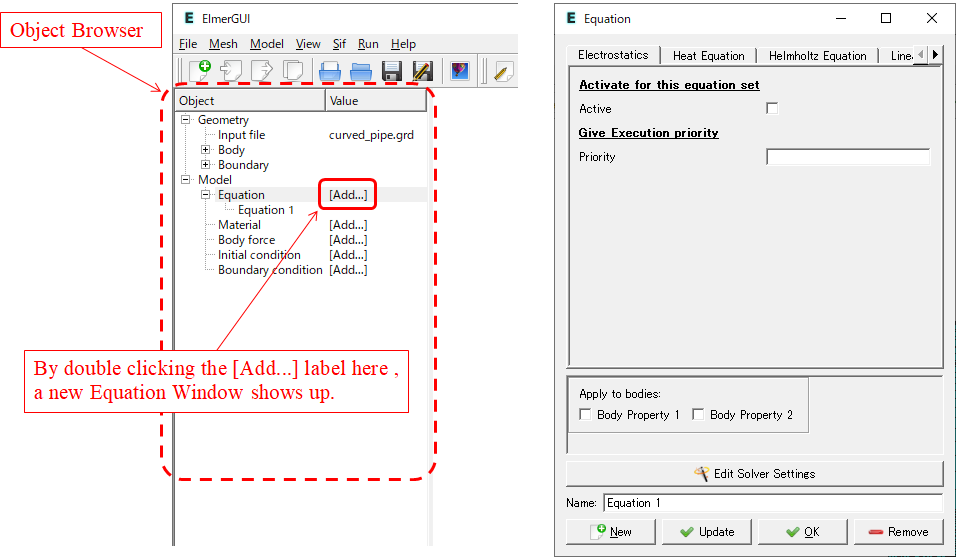
\includegraphics[scale=0.5]{images/equation.png}
\caption{Adding a new Equation.}
\label{fig:equation}
\end{center}
\end{figure}

Once the PDE-system has been defined by activating the individual equations, the numerical
methods and parameters can be selected and tuned in Solver Settings Window (Figure \ref{fig:solversettings}) which appears by pressing the ``Edit Solver Settings'' button.
The name of the PDE-system is defined in the line edit box with label ``Name''. After pressing
the OK-button, the equation remains visible and editable under the Model menu. 
It is also possible to show and edit the Equation Window by double clicking the name of the equation under ``Equation'' item in Object Browser.

\begin{figure}[htb]
\begin{center}
 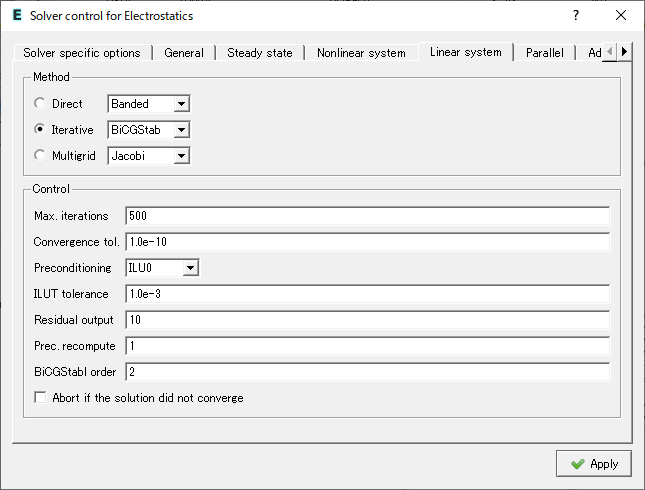
\includegraphics[scale=0.5]{images/solversettings.png}
\caption{Solver Settings Window.}
\label{fig:solversettings}
\end{center}
\end{figure}

If some of checkboxes in ``Apply to bodies'' in the Equation Window are checked, this equation is applied to these bodies. 
Another way to apply a equation to a body without using Equation Window is by holding down the SHIFT-key while double clicking one of its surfaces (or simply double clicking the surface while ``Set body properties'' button in the toolbar is pressed down).
As shown in Figure \ref{fig:bodypropertyeditor}, a Body Property Editor will then appear,
listing all possible attributes that can be apply to the selection. The Body Property Editor will show up also by double clicking the body name under ``Body'' item in the Object Browser. 


\begin{figure}[htb]
\begin{center}
 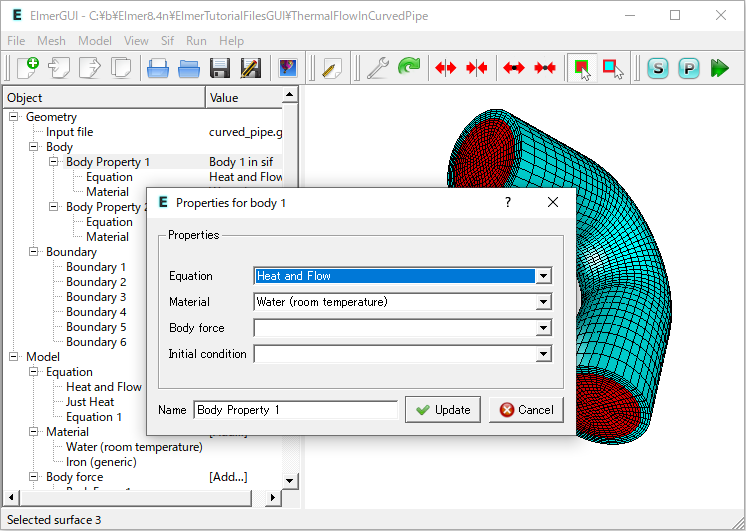
\includegraphics[scale=0.5]{images/bodyproperties.png}
\caption{Body Property Editor is activated by holding down the SHIFT key while double
clicking a surface.}
\label{fig:bodypropertyeditor}
\end{center}
\end{figure}

\section{Material menu}

The next menu is related to material and model parameters:
\menu{Model}{Material}
This menu will be used to generate the ``Material'' blocks in a solver
input file.

\noindent In order to define a material parameter set and apply it to bodies, choose
\dynmenu{Model}{Material}{Add...}
\noindent or clicking [Add...] label next to ``Material'' item in Object Browser. This will open a Material Window (Figure \ref{fig:material}).

\begin{figure}[htb]
\begin{center}
 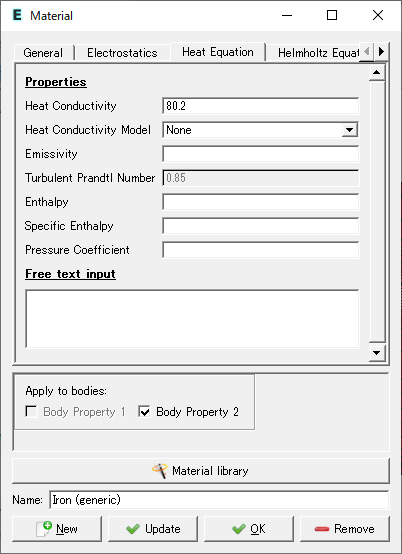
\includegraphics[scale=0.5]{images/material.png}
\caption{Material Window.}
\label{fig:material}
\end{center}
\end{figure}

Again, it is possible to apply the material to a body by holding down the
SHIFT-key while double clicking one of its surfaces (or simply double clicking the surface while ``Set body properties'' button in the toolbar is pressed down).
A Body Property Editor will then appear,
listing all possible attributes that can be apply to the selection. The Body Property Editor will show up also by double clicking the body name under ``Body'' item in the Object Browser. 

\vskip2mm

{\bf Note}: The value of density should always be defined in the ``General'' tab. This
field should never be left undefined.

\vskip2mm

{\bf Note}: If you set focus in a line edit box of a dynamical menu and press Enter, a small
text edit dialog will pop up. This allows the input of more complicated expressions
than just constants. As an example, go to {\it Model $\rightarrow$ Material} and choose
{\it Add...} Place the cursor in the ``Heat conductivity'' line edit box of ``Heat
equation'' and press Enter. You can then define the heat conductivity
as a function of temperature as a piecewise linear function. An example is show in
Figure~\ref{fig_editbox}. In this case, the heat conductivity gets value 10 if the temperature is less
than 273 degrees. It then rises from 10 to 20 between 273 and 373 degrees, and
remains constant 20 above 373 degrees.

\begin{figure}[htb]
	\begin{center}
		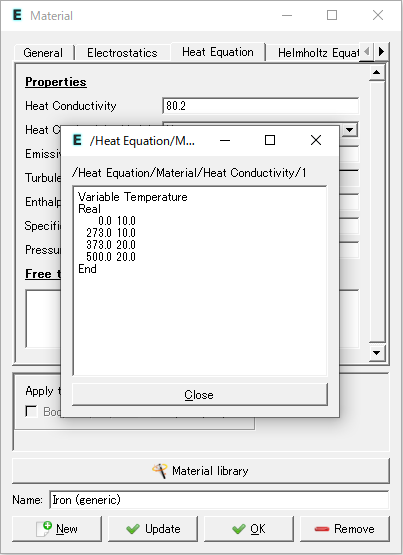
\includegraphics[scale=0.5]{images/textedit.png}
		\caption{Text edit extension of a line edit box is activated by pressing Enter.}
		\label{fig_editbox}
	\end{center}
\end{figure}

If the user presses SHIFT and F1, a tooltip for the active widget will be displayed as shown in Figure \ref{fig:tooltip}.

\begin{figure}[htb]
	\begin{center}
		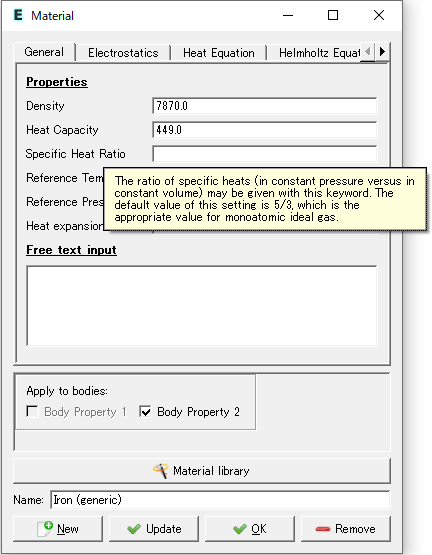
\includegraphics[scale=0.5]{images/tooltip.png}
		\caption{Tooltips are shown by holding down the SHIFT and F1 keys.}
		\label{fig:tooltip}
	\end{center}
\end{figure}

\section{Body force menu}

The next menu in the list is
\menu{Model}{Body force}
 This menu is used to construct the ``Body force'' blocks in a
solver input file.

\noindent Again, choose
\dynmenu{Model}{Body force}{Add...}
\noindent to define a set of body forces and apply it to the bodies. It is also possible to click [Add...] label next to ``Body force'' item in Object Browser. This will open a Body Force Window (Figure \ref{fig:bodyforce}).

\begin{figure}[htb]
\begin{center}
 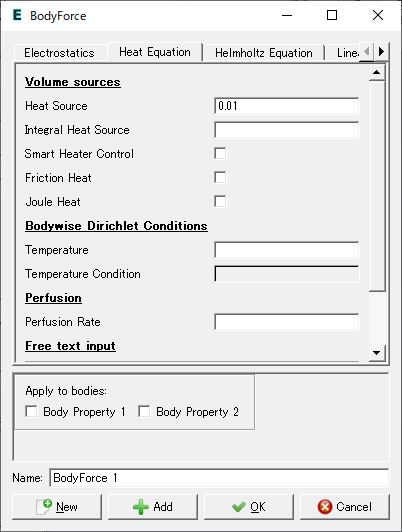
\includegraphics[scale=0.5]{images/bodyforce.png}
\caption{Body Force Window.}
\label{fig:bodyforce}
\end{center}
\end{figure}

\section{Initial condition menu}

The last menu related to body properties is
\menu{Model}{Initial condition}
\noindent 
Once again, choose
\dynmenu{Model}{Initial condition}{Add...}
\noindent to define a set of initial conditions and apply it to the bodies. It is also possible to click [Add...] label next to ``Initial condition'' item in Object Browser. This will open an Initial Condition Window (Figure \ref{fig:initialcondition}).

This menu is used to construct the ``Initial condition'' blocks in a
solver input file.

\begin{figure}[htb]
\begin{center}
 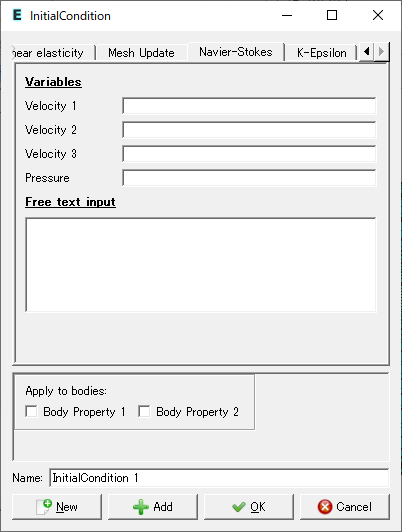
\includegraphics[scale=0.5]{images/initialcondition.png}
\caption{Initial Condition Window.}
\label{fig:initialcondition}
\end{center}
\end{figure}

\section{Boundary condition menu}

Finally, there is a menu entry for setting up the boundary conditions:
\menu{Model}{Boundary condition}
\noindent Choose
\dynmenu{Model}{Boundary condition}{Add...}
\noindent to define a set of boundary conditions and apply them to boundaries. It is also possible to click [Add...] label next to ``Boundary condition'' item in Object Browser. This will open a Boundary Condition Window (Figure \ref{fig:boundarycondition}). 

\begin{figure}[htb]
\begin{center}
 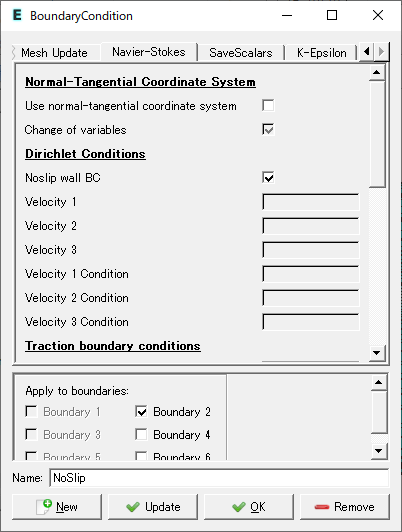
\includegraphics[scale=0.5]{images/boundarycondition.png}
\caption{Boundary Condition Window.}
\label{fig:boundarycondition}
\end{center}
\end{figure}

It is possible to apply a boundary condition to a boundary by holding down 
the \texttt{Alt} or \texttt{AltGr}-key while double clicking a surface or edge. (or simply double clicking the surface or edge while ``Set boundary properties'' button in the toolbar is pressed down).
As shown in Figure \ref{fig:boundarypropertyeditor}, a Boundary Property Editor will appear, listing all possible conditions that can be applyed to the selection. The Boundary Property Editor will show up also by double clicking the boundary name under ``Boundary'' item in the Object Browser. 

Choose a condition from the combo box and finally press \texttt{Ok}.
\begin{figure}[htb]
\begin{center}
 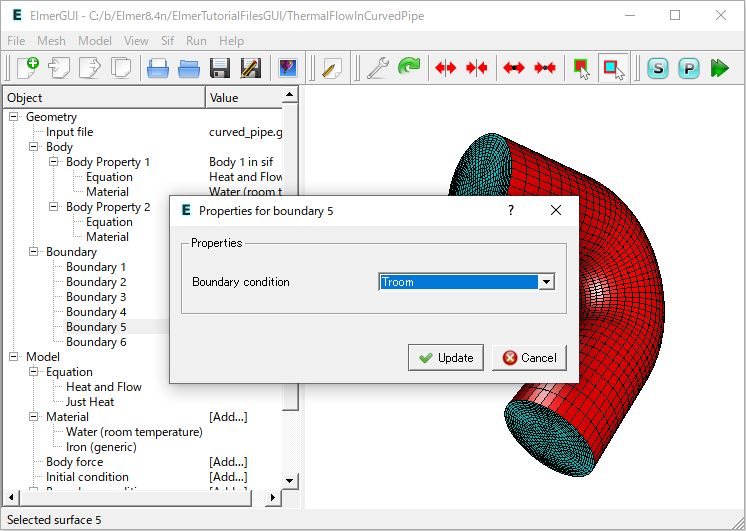
\includegraphics[scale=0.5]{images/boundaryproperties.png}
\caption{Boundary Property Editor activated by holding down the \texttt{AltGr} key while double
clicking a surface.}
\label{fig:boundarypropertyeditor}
\end{center}
\end{figure}

\chapter{Utility functions}

\section{Boundary division and unification}

Some of the input file formats listed in Table \ref{table:inputfiles} are not perhaps so well suited for
FE-calculations, even though widely used. The .stl format (stereo lithography format),
for example, is by definition unable to distinguish between different boundary parts
with different attributes. Moreover, the format approximates the boundary by disconnected
triangles that do not fulfill the usual FE-compatibility conditions.

In order to deal with formats like .stl, ElmerGUI provides a minimal set of tools for
boundary division and unification. The division is based on ``sharp edge detection''.
An edge between two boundary elements is considered sharp, if the angle between the
normals exceeds a certain value (20 degrees by default). The sharp edges are then used
as a mortar to divide the surface into parts. The user may perform a sharp edge detection
and boundary division from the Mesh menu by choosing
\menu{Mesh}{Divide surface...}
\noindent In 2D the corresponding operation is
\menu{Mesh}{Divide edge...}
\noindent The resulting parts are enumerated starting from the first free index.

Sometimes, the above process produces far too many distinct parts, which eventually
need to be (re)unified. This can be done by selecting a group of surfaces by holding
down the CTRL-key while double clicking the surfaces and choosing
\menu{Mesh}{Unify surface...}
\noindent The same operation in 2D is
\menu{Mesh}{Unify edge...}
The result will inherit the smallest index from the selected group.

\noindent The sharp edges that do not belong to a closed loop may be removed by
\menu{Mesh}{Clean up}
\noindent This operation has no effect on the boundary division, but sometimes it makes
the result look better.

\section{Saving pictures}

The model drawn on the display area may be scanned into a 24-bit RGB image and saved in
several picture file formats:
\menu{File}{Save picture as...}
\noindent The function supports .bmp, .jpg, .png, .pbm, .pgm, and .ppm file extensions.

\section{View menu}

The View menu provides several utility functions for controlling the visual behavior
of ElmerGUI. The function names should be more or less self explanatory.

\chapter{Solver input files}

The contents of the Model menu are passed to the solver in the form of a solver
input file. A solver input file is generated by choosing
\menu{Sif}{Generate}
\noindent The contents of the file are editable in Solver Input File Window which shows up by choosing
\menu{Sif}{Edit...}
As shown in Figure  \ref{fig:sifwindow}, two types of syntax highlighting are available in Solver Input File Window from the menu on it:
\menu{Preference}{Syntax highlighting}
\noindent Font can be also changed by 
\menu{Preference}{Font}

\begin{figure}[htb]
	\begin{center}
		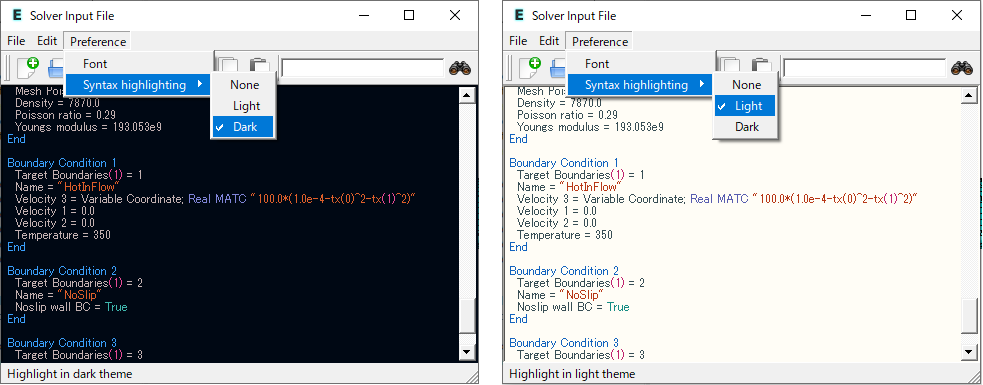
\includegraphics[scale=0.5]{images/sifwindow.png}
		\caption{Syntax highlighting in Solver Input File Window}
		\label{fig:sifwindow}
	\end{center}
\end{figure}

\noindent The new sif file needs to be saved before it becomes active. The recommended
method is
\menu{File}{Save project}
\noindent In this way, also the current mesh and project files get saved in the
same directory, avoiding possible inconsistencies later on.
\vspace{3mm}\\
{\bf Note}: The previous versions of ElmerGUI automatically generated (i.e. overwrote) solver input file when saving or loading the project or mesh and it was inconvenient when manually modifying solver input file. Current version of ElmerGUI does not generate solver input file automatically when saving/loading project or mesh.

\chapter{Solution and post processing}

\section{Running the solver}

Once the solver input file has been generated and the project has been saved,
it is possible to actually solve the problem:
\menu{Run}{Start solver}
\noindent This will launch either a single process for ElmerSolver (scalar solution)
or multiple MPI-processes for ElmerSolver\_mpi (parallel solution) depending on the
definitions in
\menu{Run}{Parallel settings...}


\begin{figure}[htb]
\begin{center}
 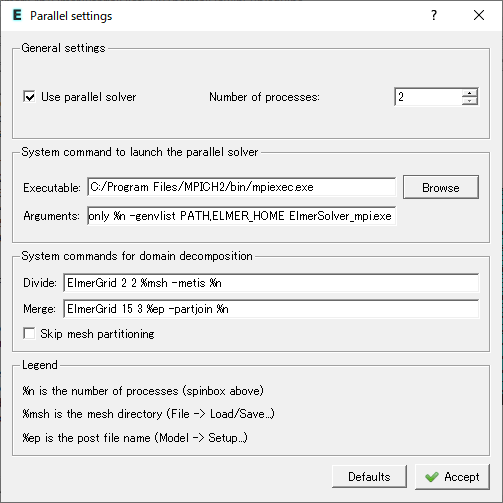
\includegraphics[scale=0.5]{images/parallelsettings.png}
\caption{Parallel Settings Window.}
\label{fig:parallelsettings}
\end{center}
\end{figure}

As shown in Figure \ref{fig:parallelsettings}, the parallel menu has three group boxes. Usually, the user is supposed to touch
only the ``General settings'' group and select the number of processes to execute.
The two remaining groups deal with system commands to launch MPI-processes and
external tools for domain decomposition.  The parallel menu is greyed out if
ElmerSolver\_mpi is not present at start-up.

When the solver is running, there is a log window and a convergence monitor
from which the iteration may be followed. In case of divergence or other troubles,
the solver may be terminated by choosing
\menu{Run}{Kill solver}

Once the solver has started, Solver Log Window will appears to show the log. Solver Log Window also has menus for syntax highlighting and font selection like Solver Input File Window. 

The solver will finally write a result file for postprocessor in the project directory.
The name of the result file is defined in
\menu{Model}{Setup...}

It may be tiresome to generate solver input file, save the project then run solver every time you make a slight modification in conditions. ``Generate, save and run'' button (a button with green doubled triangle) in the toolbar enables these three actions by one clicking of the button. This will be helpful to quickly run the case modified via GUI.
A similar button - ``Save and run'' button (a button with single green triangle) is also in Solver Input File Window. This button saves the solver input file and the project then runs the solver. This will be helpful to quickly run the case manually modified via Solver Input File Window. 
These buttons are shown in Figure \ref{fig:quickbuttons}.

\begin{figure}[htb]
	\begin{center}
		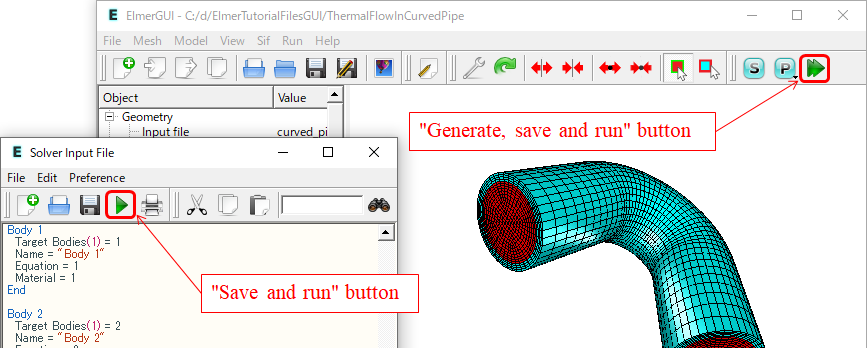
\includegraphics[scale=0.5]{images/quickrunbuttons.png}
		\caption{Buttons for quick run.}
		\label{fig:quickbuttons}
	\end{center}
\end{figure}
\section{Post processing}

If the path settings are set properly, ElmerGUI can call Paraview directly from
\menu{Run}{Start ParaView}
Note that you may always open Paraview also independently from ElmerGUI. 

ElmerGUI still also includes calling possibility of the obsolete ElmerPost visualization tool.
It will with time be eliminated also from the GUI. 


%includes callprovides two different post processors for drawing, displaying, and manipulating the results.

The first alternative is activated from
\menu{Run}{Start ElmerPost}
\noindent This will launch ElmerPost, which will read in the result file and displays a contour plot representing the solution. If the results were produced by the parallel solver, the domain decomposition used in the calculations will be shown. Because ElmerPost can handle only ``.ep'' file, you should specify the Post file in Simulation section of Setup Window with extension of ``.ep'' such like ``case.ep'' while it is ``case.vtu'' by default.

The second post processor is based on the Visualization Toolkit, VTK. It is activated from
\menu{Run}{ElmerVTK}
\noindent A new window will then pop up, providing methods for drawing surfaces, contours,
vectors, and stream lines.

In the toolbar of ElmerGUI main window, there is a button for launching postprocessor. The postprocessor to be launched can be selected by long pressing the button as shown in Figure \ref{fig:prostprocessors}.  
\begin{figure}[htb]
	\begin{center}
		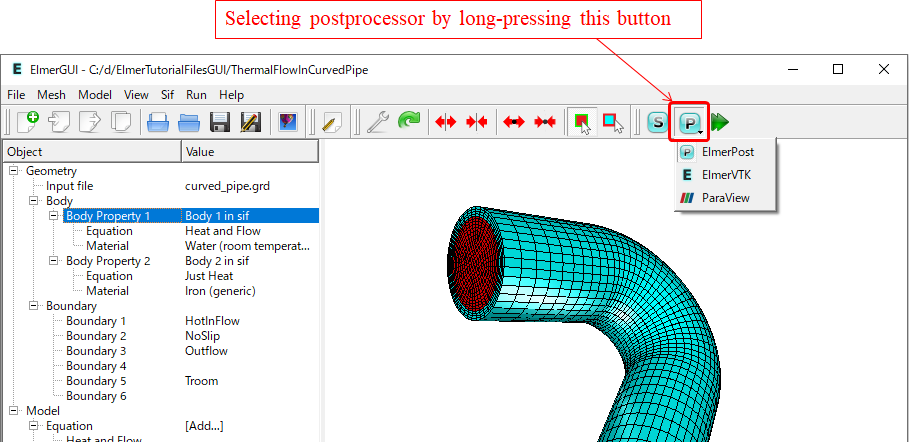
\includegraphics[scale=0.5]{images/postprocessors.png}
		\caption{Selecting postprocessor in toolbar.}
		\label{fig:prostprocessors}
	\end{center}
\end{figure}

% No longer supported

\begin{comment}
\subsection{Python interface}

If ElmerGUI has been compiled with PythonQt-support, there is a Python console
available for scripting. The console is located under the Edit-menu:
\menu{Edit}{PythonQt console...}
\noindent The console provides access to the following classes:
\begin{footnotesize}
\begin{verbatim}
egp             // ElmerGUI post processor
matc            // MATC language interpreter
preferences     // controls for preferences
surfaces        // controls for surface plots
vectors	        // controls for vector fields
isoContours     // controls for isocontours
isoSurfaces     // controls for isosurfaces
streamLines     // controls for streamlines
colorBar        // cotrols for the colorbar
timeStep        // controls for transient results
text            // text annotation
\end{verbatim}
\end{footnotesize}

Each of the above classes provides a number of useful methods for data and display
manipulation. To fix ideas, suppose that we want to read in the result file ``case.ep''
and display the temperature fields as a semi transparent surface plot. The commands
to execute are then the following (more examples can be found in section 7.3.3):
\begin{footnotesize}
\begin{verbatim}
py> egp.ReadPostFile("case.ep")
py> egp.SetSurfaces(True)
py> surfaces.SetFieldName("Temperature")
py> surfaces.SetOpacity(50)
py> egp.Redraw()
\end{verbatim}
\end{footnotesize}

\subsection{Public methods}
Interface version 0.2:
\begin{footnotesize}
\begin{verbatim}
class egp:
  bool MatcCmd(QString);                         // evaluate MATC cmd
  void domatcSlot();                             // flush MATC console

  void SetPostFileStart(int);                    // first time step
  void SetPostFileEnd(int);                      // last time step
  bool ReadPostFile(QString);                    // read result file

  void Render();                                 // render
  void ResetCamera();                            // reset camera
  void Redraw();                                 // redraw actors
  void ResetAll();                               // reset view

  void SetSurfaces(bool);                        // show/hide surfaces
  void SetVectors(bool);                         // show/hide vectors
  void SetIsoContours(bool);                     // show/hide isocontours
  void SetIsoSurfaces(bool);                     // show/hide isosurfaces
  void SetStreamLines(bool);                     // show/hide streamlines
  void SetColorBar(bool);                        // show/hide colorbar
  void SetMeshPoints(bool);                      // show/hide/nodes
  void SetMeshEdges(bool);                       // show/hide edges
  void SetFeatureEdges(bool);                    // show/hide f-edges
  void SetAxes(bool);                            // show/hide axes
  void SetText(bool);                            // show/hide text

  bool GetClipAll();                             // is clipping on?
  void SetClipAll(bool);                         // clipping on/off
  void SetClipPlaneOx(double);                   // clip plane origin
  void SetClipPlaneOy(double);                   // clip plane origin
  void SetClipPlaneOz(double);                   // clip plane origin
  void SetClipPlaneNx(double);                   // clip plane normal
  void SetClipPlaneNy(double);                   // clip plane normal
  void SetClipPlaneNz(double);                   // clip plane normal

  double GetCameraDistance();                    // get camera distance
  void SetCameraDistance(double);                // set camera distance
  double GetCameraPositionX();                   // get camera position
  double GetCameraPositionY();                   // get camera position
  double GetCameraPositionZ();                   // get camera position
  void SetCameraPositionX(double);               // set camera position
  void SetCameraPositionY(double);               // set camera position
  void SetCameraPositionZ(double);               // set camera position
  double GetCameraFocalPointX();                 // get focal point
  double GetCameraFocalPointY();                 // get focal point
  double GetCameraFocalPointZ();                 // get focal point
  void SetCameraFocalPointX(double);             // set focal point
  void SetCameraFocalPointY(double);             // set focal point
  void SetCameraFocalPointZ(double);             // set focal point
  void CameraDolly(double);                      // dolly
  void CameraRoll(double);                       // roll
  void CameraAzimuth(double);                    // azimuth
  void CameraYaw(double);                        // yaw
  void CameraElevation(double);                  // elevation
  void CameraPitch(double);                      // pitch
  void CameraZoom(double);                       // zoom
  void SetCameraRoll(double);                    // set roll
  void SetInitialCameraPosition();               // set initial position

  void RotateX(double);                          // rotate visible actors
  void RotateY(double);                          // rotate visible actors
  void RotateZ(double);                          // rotate visible actors
  void SetOrientation(double, double, double);   // set orientation
  void SetPositionX(double);                     // set position
  void SetPositionY(double);                     // set position
  void SetPositionZ(double);                     // set position
  void SetPosition(double, double, double);      // set position
  void AddPosition(double, double, double);      // add position
  void SetOrigin(double, double, double);        // set origin
  void SetScaleX(double);                        // set scale
  void SetScaleY(double);                        // set scale
  void SetScaleZ(double);                        // set scale
  void SetScale(double, double, double);         // set scale
  double GetLength();                            // get model size
  double GetNofNodes();                          // get nof nodes
  double GetMinX();                              // bounding box
  double GetMaxX();                              // bounding box
  double GetMinY();                              // bounding box
  double GetMaxY();                              // bounding box
  double GetMinZ();                              // bounding box
  double GetMaxZ();                              // bounding box

  bool SavePngFile(QString);                     // save image file

  void SetBgColor(double, double, double);       // bg color (RGB: 0..1)

class matc:
  bool SetCommand(QString);                      // Enter MATC cmd

class preferences:
  void UseSurfaceMeshForPoints(bool);            // nodes of surface mesh
  void UseVolumeMeshForPoints(bool);             // nodes of volume mesh
  void SetPointSize(int);                        // set node point size
  void SetPointQuality(int);                     // set node point quality
  void UseClipPlaneForPoints(bool);              // clip nodes
  void UseSurfaceMeshForEdges(bool);             // edges of surface mesh
  void UseVolumeMeshForEdges(bool);              // edges of volume mesh
  void UseTubeFilterForEdges(bool);              // use tube filter
  void UseClipPlaneForEdges(bool);               // clip edges
  void SetLineWidthForEdges(int);                // edge line width
  void SetTubeQualityForEdges(int);              // edge tube quality
  void SetTubeRadiusForEdges(int);               // edge tube radius
  void UseSurfaceMeshForFeatureEdges(bool);      // surface mesh: f-edges
  void UseVolumeMeshForFeatureEdges(bool);       // volume mesh: f-edges
  void UseTubeFilterForFeatureEdges(bool);       // use tube filter
  void UseClipPlaneForFeatureEdges(bool);        // clip f-edges
  void DrawBoundaryEdges(bool);                  // draw boundary edges
  int GetFeatureAngle();                         // get feature angle
  void SetFeatureAngle(int);                     // set feature angle
  void SetLineWidthForFeatureEdges(int);         // f-edge line width
  void SetTubeQualityForFeatureEdges(int);       // f-edge tube quality
  void SetTubeRadiusForFeatureEdges(int);        // f-edge tube radius
  void SetClipPlaneOx(double);                   // clip plane origin
  void SetClipPlaneOy(double);                   // clip plane origin
  void SetClipPlaneOz(double);                   // clip plane origin
  void SetClipPlaneNx(double);                   // clip plane normal
  void SetClipPlaneNy(double);                   // clip plane normal
  void SetClipPlaneNz(double);                   // clip plane normal

class surfaces:
  QString GetFieldName();                        // get field name
  bool SetFieldName(QString);                    // set field name
  void SetMinVal(double);                        // set minimum
  void SetMaxVal(double);                        // set maximum
  void KeepLimits(bool);                         // keep limits
  void SetComputeNormals(bool);                  // shade model
  void SetFeatureAngle(int);                     // feature angle
  void SetOpacity(int);                          // set opacity
  void SetClipPlane(bool);                       // set clipping

class vectors:
  QString GetFieldName();                        // get field name
  bool SetFieldName(QString);                    // set field name
  void SetMinVal(double);                        // set minimum
  void SetMaxVal(double);                        // set maximum
  void KeepLimits(bool);                         // keep limits
  void SetComputeNormals(bool);                  // shade model
  void SetFeatureAngle(int);                     // feature angle
  void SetOpacity(int);                          // set opacity
  void SetClipPlane(bool);                       // set clipping

class isoContours:
  QString GetFieldName();                        // get field name
  QString GetColorName();                        // get color name
  bool SetFieldName(QString);                    // set field name
  bool SetColorName(QString);                    // set color name
  void SetMinFieldVal(double);                   // set min value
  void SetMaxFieldVal(double);                   // set max value
  void SetContours(int);                         // set nof contours
  void KeepFieldLimits(bool);                    // keep limits
  void SetMinColorVal(double);                   // set color min
  void SetMaxColorVal(double);                   // set color max
  void KeepColorLimits(bool);                    // keep color limits
  void UseTubeFilter(bool);                      // use tube filter
  void UseClipPlane(bool);                       // set clipping on/off
  void SetLineWidth(int);                        // set line width
  void SetTubeQuality(int);                      // set tube quality
  void SetTubeRadius(int);                       // set tube radius

class isoSurfaces:
  QString GetFieldName();                        // get field name
  QString GetColorName();                        // get color name
  bool SetFieldName(QString);                    // set field name
  bool SetColorName(QString);                    // set color name
  void SetMinFieldVal(double);                   // set min value
  void SetMaxFieldVal(double);                   // set max value
  void SetContours(int);                         // nof contours
  void KeepFieldLimits(bool);                    // keep limits
  void SetMinColorVal(double);                   // set color min
  void SetMaxColorVal(double);                   // set color max
  void KeepColorLimits(bool);                    // keep color limits
  void ComputeNormals(bool);                     // shade model
  void UseClipPlane(bool);                       // set clpping on/off
  void SetFeatureAngle(int);                     // set feature angle
  void SetOpacity(int);                          // set opacity

class streamLines:
  QString GetFieldName();                        // get field name
  QString GetColorName();                        // get color name
  bool SetFieldName(QString);                    // set field name
  bool SetColorName(QString);                    // set color name
  void SetMaxTime(double);                       // max time
  void SetStepLength(double);                    // step length
  void SetThreads(int);                          // nof threads
  void SetIntegStepLength(double);               // integ. step length
  void UseSurfaceMesh(bool);                     // use forface mesh
  void UseVolumeMesh(bool);                      // use volume mesh
  void IntegrateForwards(bool);                  // integrate forwards
  void IntegrateBackwards(bool);                 // integrate backwards
  void SetMinColorVal(double);                   // color min val
  void SetMaxColorVal(double);                   // color max value
  void KeepColorLimits(bool);                    // keep color limits
  void DrawLines(bool);                          // draw using lines
  void DrawRibbons(bool);                        // draw using ribbons
  void SetLineWidth(int);                        // line width
  void SetRibbonWidth(int);                      // ribbon width
  void UseSphereSource(bool);                    // use sphere source
  void UseLineSource(bool);                      // use line source
  void UsePointSource(bool);                     // use point source
  void SetSphereSourceX(double);                 // sphere origin
  void SetSphereSourceY(double);                 // sphere origin
  void SetSphereSourceZ(double);                 // sphere origin
  void SetSphereSourceRadius(double);            // sphere radius
  void SetSphereSourcePoints(int);               // nof pts in sphere
  void SetLineSourceStartX(double);              // line start point
  void SetLineSourceStartY(double);              // line start point
  void SetLineSourceStartZ(double);              // line start point
  void SetLineSourceEndX(double);                // line end point
  void SetLineSourceEndY(double);                // line end point
  void SetLineSourceEndZ(double);                // line end point
  void SetLineSourcePoints(int);                 // nof pts on line

class colorBar:
  bool SetFieldName(QString);                    // set field name
  void UseHorizontalLayout(bool);                // horizontal layout
  void UseVerticalLayout(bool);                  // vertical layout
  void AnnotateFieldName(bool);                  // annotate field name
  void SetLabels(int);                           // set nof labels
  void SetLineWidth(double);                     // set line width
  void SetLength(double);                        // set bar length

class timeStep:
  void SetCurrent(int);                          // set current step
  void SetStart(int);                            // set first step
  void SetStop(int);                             // set last step
  void SetIncrement(int);                        // set increment
  void SetMatcCmd(QString);                      // set MATC cmd
  void RegenerateBeforeDrawing(bool);            // regenerate actors
  void SaveFrames(bool);                         // save frames
  void SetSaveDirectory(QString);                // set save dir
  void Loop();                                   // toggle looping
  bool IsLooping();                              // is loop on?
  void DrawCurrent();                            // draw current frame

class text:
  void SetMessage(QString);                      // annotation
  void SetPosX(int);                             // set x-position
  void SetPosy(int);                             // set y-position
  void SetLeft();                                // justification
  void SetCentered();                            // justification
  void SetRight();                               // justification
  void SetSize(int);                             // font size
  void SetBold(bool);                            // bold
  void SetItalic(bool);                          // italic
  void SetShadow(bool);                          // shadow
  void SetRed(double);                           // red (0..1)
  void SetGreen(double);                         // green (0..1)
  void SetBlue(double);                          // blue (0..1)
  void SetRGB(double, double, double);           // text color (RGB: 0..1)
\end{verbatim}
\end{footnotesize}

\subsection{Example scripts}

The exampels below are executed from the PythonQt-console as
\begin{footnotesize}
\begin{verbatim}
py> execfile("sample.py")
\end{verbatim}
\end{footnotesize}
where ``sample.py'' is a text file containing the script to run.

\vskip5mm
\noindent{\bf Read in results}
\begin{footnotesize}
\begin{verbatim}
egp.ReadPostFile("case.ep")
\end{verbatim}
\end{footnotesize}

\vskip5mm
\noindent{\bf Set orientation}
\begin{footnotesize}
\begin{verbatim}
egp.ReadPostFile("case.ep")
egp.SetSurfaces(True)
egp.SetOrientation(45, 45, 0)
egp.SetInitalCameraPosition()
\end{verbatim}
\end{footnotesize}

\vskip5mm
\noindent{\bf Visualize temperature on surfaces}
\begin{footnotesize}
\begin{verbatim}
egp.ReadPostFile("case.ep")
egp.SetSurfaces(True)
egp.SetOrientation(45, 45, 0)
egp.SetInitalCameraPosition()
surfaces.SetFieldName("Temperature")
egp.Redraw()
\end{verbatim}
\end{footnotesize}


\vskip5mm
\noindent{\bf Rotate object}
\begin{footnotesize}
\begin{verbatim}
import time
egp.ReadPostFile("case.ep")
egp.SetSurfaces(True)
for i in range (180):
        egp.RotateY(2.0)
        egp.ResetCamera()
        egp.Render()
        time.sleep(0.1)
\end{verbatim}
\end{footnotesize}


\vskip5mm
\noindent{\bf Traveling isosurface}
\vskip5mm
\noindent The following script makes an iso surface ($z=const.$) travel through the model
in 100 steps. The surface is colored according to the temperature field. The model it self
is drawn transparent.
\begin{footnotesize}
\begin{verbatim}
import time
egp.ReadPostFile("case.ep")
egp.SetSurfaces(True)
egp.SetIsoSurfaces(True)
egp.SetFeatureEdges(True)
preferences.SetFeatureAngle(45)
surfaces.SetFieldName("Null")
surfaces.SetOpacity(20)
isoSurfaces.SetFieldName("nodes_z")
isoSurfaces.SetColorName("Temperature")
isoSurfaces.SetContours(1)
isoSurfaces.KeepFieldLimits(True)
egp.SetOrientation(45, 45, 0)
egp.ResetCamera()
egp.Render()
zmin = egp.GetMinZ()
zmax = egp.GetMaxZ()
for i in range(100):
    z = zmin+(float(i)/100.0)*(zmax-zmin)
    isoSurfaces.SetMinFieldVal(z)
    isoSurfaces.SetMaxFieldVal(z)
    egp.Redraw()
    time.sleep(0.05)
\end{verbatim}
\end{footnotesize}


\vskip5mm
\noindent{\bf Rotate and save frames}
\begin{footnotesize}
\begin{verbatim}
egp.ReadPostFile("case.ep")
egp.SetSurfaces(True)
for i in range (180):
        egp.RotateY(2.0)
        egp.ResetCamera()
        egp.Render()
        egp.SavePngFile("frame" + str(i) + ".png")
\end{verbatim}
\end{footnotesize}

\vskip5mm
\noindent{\bf Preparing and playing back video clips}

\vskip5mm

\noindent With ffmpeg (see ffmpeg's manuals for more accurate controls):
\begin{footnotesize}
\begin{verbatim}
$ ffmpeg -b 1000000 -i frame%d.png example.avi
\end{verbatim}
\end{footnotesize}
With mencoder (see mencoder's manuals for better controls):
\begin{footnotesize}
\begin{verbatim}
$ mencoder -ovc lavc -mf type=png:fps=25 -o example.avi mf://frame%d.png
\end{verbatim}
\end{footnotesize}
Playback with mplayer (choose appropriate frame rate):
\begin{footnotesize}
\begin{verbatim}
$ mplayer -fps 50 example.avi
\end{verbatim}
\end{footnotesize}

\subsection{ECMAScript interface}

In addition to Python, it is possible to use Qt's internal ECMAScript engine for scripting. The ECMAScript console is activated from
the Edit menu as:
\menu{Edit}{ECMAScript console...}
The ECMAScript interface provides access to the same classes and methods
as the Python interface. However, users familiar with e.g. JavaScript (from
which ECMAScript has been derived and standardized) may find the ECMAScript interface more comfortable.

ECMAScript files are executed from the console by entering the command
\begin{footnotesize}
\begin{verbatim}
qs> egp.Execute("script.qs")
\end{verbatim}
\end{footnotesize}

The above examples for Python translate to the following ECMAScript files:

\vskip5mm
\noindent{\bf Read in results}
\begin{footnotesize}
\begin{verbatim}
egp.ReadPostFile("case.ep")
\end{verbatim}
\end{footnotesize}

\vskip5mm
\noindent{\bf Set orientation}
\begin{footnotesize}
\begin{verbatim}
egp.ReadPostFile("case.ep")
egp.SetSurfaces(true)
egp.SetOrientation(45, 45, 0)
egp.SetInitalCameraPosition()
\end{verbatim}
\end{footnotesize}

\vskip5mm
\noindent{\bf Visualize temperature on surfaces}
\begin{footnotesize}
\begin{verbatim}
egp.ReadPostFile("case.ep")
egp.SetSurfaces(true)
egp.SetOrientation(45, 45, 0)
egp.SetInitalCameraPosition()
surfaces.SetFieldName("Temperature")
egp.Redraw()
\end{verbatim}
\end{footnotesize}

\vskip5mm
\noindent{\bf Rotate object}
\begin{footnotesize}
\begin{verbatim}
egp.ReadPostFile("case.ep")
egp.SetSurfaces(true)
for(var i = 0; i < 180; i++)
{
   egp.RotateY(2.0)
   egp.ResetCamera()
   egp.Render()
}
\end{verbatim}
\end{footnotesize}

\vskip5mm
\noindent{\bf Traveling isosurface}
\begin{footnotesize}
\begin{verbatim}
egp.ReadPostFile("case.ep")
egp.SetSurfaces(true)
egp.SetIsoSurfaces(true)
egp.SetFeatureEdges(true)
preferences.SetFeatureAngle(45)
surfaces.SetFieldName("Null")
surfaces.SetOpacity(20)
isoSurfaces.SetFieldName("nodes_z")
isoSurfaces.SetColorName("Temperature")
isoSurfaces.SetContours(true)
isoSurfaces.KeepFieldLimits(true)
egp.SetOrientation(45, 45, 0)
egp.ResetCamera()
egp.Render()
var zmin = egp.GetMinZ()
var zmax = egp.GetMaxZ()
for(var i = 0; i < 100; i++)
{
   var z = zmin + i/100.0 * (zmax-zmin)
   isoSurfaces.SetMinFieldVal(z)
   isoSurfaces.SetMaxFieldVal(z)
   egp.Redraw()
}
\end{verbatim}
\end{footnotesize}

\vskip5mm
\noindent{\bf Rotate and save frames}
\begin{footnotesize}
\begin{verbatim}
egp.ReadPostFile("case.ep")
egp.SetSurfaces(true)
for(var i = 0; i < 180; i++)
{
    egp.RotateY(2.0)
    egp.ResetCamera()
    egp.Render()
    egp.SavePngFile("frame" + i + ".png")
}
\end{verbatim}
\end{footnotesize}

\vskip5mm
\noindent{\bf Visualize transient results and save frames}
\begin{footnotesize}
\begin{verbatim}
// Result file:
//--------------
var file = "case.ep";
var start = 1;
var end = 50;

// Read in transient results:
//----------------------------
egp.SetPostFileStart(start);
egp.SetPostFileEnd(end);
egp.ReadPostFile(file);

// Select methods:
//-----------------
egp.SetSurfaces(true);
egp.SetFeatureEdges(true);
egp.SetText(true);

// Select scalar field:
//----------------------
surfaces.SetFieldName("Temperature");

// Loop over time steps:
//-----------------------
for(var index = start; index <= end; index++) {
        timeStep.SetCurrent(index);
        text.SetMessage("Time step = " + index);
        egp.Redraw();
        egp.SavePngFile("frame" + index + ".png");
}
\end{verbatim}
\end{footnotesize}

\end{comment}
